% docs/slides/preamble.tex -- 五份 deck 共享
\documentclass[aspectratio=169,11pt]{beamer}

% ==== 中文与字体 ====
\usepackage[UTF8,fontset=none]{ctex}
\usepackage{fontspec}

\IfFontExistsTF{PingFang SC}{%
  \setCJKmainfont{PingFang SC}[BoldFont=PingFang SC,ItalicFont=PingFang SC,AutoFakeSlant=0.15]
  \setCJKsansfont{PingFang SC}[ItalicFont=PingFang SC,AutoFakeSlant=0.15]
  \setCJKmonofont{PingFang SC}
}{%
  \IfFontExistsTF{Source Han Sans SC}{%
    \setCJKmainfont{Source Han Sans SC}
    \setCJKsansfont{Source Han Sans SC}
  }{%
    \IfFontExistsTF{Noto Sans CJK SC}{%
      \setCJKmainfont{Noto Sans CJK SC}
      \setCJKsansfont{Noto Sans CJK SC}
    }{%
      \setCJKmainfont{Heiti SC}
      \setCJKsansfont{Heiti SC}
    }
  }
}

\IfFontExistsTF{Helvetica Neue}{\setmainfont{Helvetica Neue}}{%
  \IfFontExistsTF{Inter}{\setmainfont{Inter}}{}}
\IfFontExistsTF{JetBrains Mono}{\setmonofont{JetBrains Mono}[Scale=0.85]}%
  {\setmonofont{Menlo}[Scale=0.85]}

% ==== 颜色 ====
\usepackage{xcolor}
\definecolor{cMain}{HTML}{1F4E79}
\definecolor{cAccent}{HTML}{E07A1F}
\definecolor{cGray}{HTML}{595959}
\definecolor{cMute}{HTML}{F4F4F4}
\definecolor{cOK}{HTML}{2E7D32}
\definecolor{cBad}{HTML}{B23A3A}
\definecolor{cWarn}{HTML}{C8A300}

% ==== 主题 ====
\usepackage{tcolorbox}
\usetheme{metropolis}
\metroset{progressbar=frametitle,numbering=fraction,block=fill}
\setbeamercolor{frametitle}{bg=cMain,fg=white}
\setbeamercolor{progress bar}{fg=cAccent,bg=cMute}
\setbeamercolor{alerted text}{fg=cAccent}
\setbeamercolor{title}{fg=cMain}

% metropolis 默认尝试 Fira Sans，未安装时 fallback 到 Latin Modern Sans。
% 这里在主题加载后显式覆盖，强制使用 macOS 上一定存在的 Helvetica Neue，
% 跟中文 PingFang 风格一致；找不到则按顺序尝试 Inter / Arial。
\IfFontExistsTF{Helvetica Neue}{%
  \setsansfont{Helvetica Neue}%
}{%
  \IfFontExistsTF{Inter}{\setsansfont{Inter}}{%
    \IfFontExistsTF{Arial}{\setsansfont{Arial}}{}}%
}

% ==== TikZ ====
\usepackage{tikz}
\usetikzlibrary{positioning,arrows.meta,fit,shapes.geometric,calc,%
  decorations.pathmorphing,backgrounds}

\tikzset{
  node-box/.style={draw=cMain,thick,rounded corners=2pt,
    minimum height=8mm,minimum width=18mm,align=center,font=\small},
  node-state/.style={draw=cMain,thick,circle,minimum size=14mm,
    align=center,font=\small},
  node-ok/.style={draw=cOK,thick,fill=cOK!10},
  node-warn/.style={draw=cWarn,thick,fill=cWarn!15},
  node-bad/.style={draw=cBad,thick,fill=cBad!10},
  % 色盲友好的状态机三态：蓝 (正常/Closed) / 橙 (告警/Open) / 灰 (中间/HalfOpen)
  % 避免 red-green 二元区分，改用 hue + lightness 双通道。
  node-state-normal/.style={draw=cMain,thick,fill=cMain!12},
  node-state-alert/.style={draw=cAccent,thick,fill=cAccent!18},
  node-state-transition/.style={draw=cGray,thick,fill=cGray!18},
  arrow/.style={-{Stealth[length=2mm]},thick,draw=cMain},
  arrow-async/.style={-{Stealth[length=2mm]},thick,dashed,draw=cGray},
  arrow-bad/.style={-{Stealth[length=2mm]},thick,draw=cBad},
  arrow-alert/.style={-{Stealth[length=2mm]},thick,draw=cAccent},
  lifeline/.style={dashed,thick,draw=cGray},
}

% ==== 代码 ====
\usepackage{listings}
\lstdefinelanguage{Go}{
  morekeywords={break,case,chan,const,continue,default,defer,else,
    fallthrough,for,func,go,goto,if,import,interface,map,package,range,
    return,select,struct,switch,type,var,nil,true,false,iota},
  morekeywords=[2]{string,int,int64,uint,uint64,bool,byte,error,context},
  sensitive=true,
  morecomment=[l]//,morecomment=[s]{/*}{*/},
  morestring=[b]",morestring=[b]`,
}
\lstdefinelanguage{LuaRedis}{
  morekeywords={and,break,do,else,elseif,end,false,for,function,if,in,
    local,nil,not,or,repeat,return,then,true,until,while},
  morekeywords=[2]{redis,call,KEYS,ARGV,tonumber,HGET,HSET,GET,SET,
    DECR,DECRBY,INCR,INCRBY,EXPIRE,PEXPIRE,ZADD,ZCARD,ZREMRANGEBYSCORE,
    EVAL,EVALSHA},
  sensitive=true,
  morecomment=[l]{--},
  morestring=[b]",morestring=[b]',
}

\lstdefinestyle{base}{
  basicstyle=\ttfamily\scriptsize,
  numbers=left,numberstyle=\tiny\color{cGray},
  keywordstyle=\color{cMain}\bfseries,
  keywordstyle=[2]\color{cAccent},
  stringstyle=\color{cOK},
  commentstyle=\color{cGray}\itshape,
  backgroundcolor=\color{cMute},
  frame=single,framerule=0pt,
  showstringspaces=false,
  breaklines=true,
  tabsize=2,
  columns=fullflexible,
}
\lstset{style=base}

% ==== 三线表与附录页码 ====
\usepackage{booktabs}
\usepackage{appendixnumberbeamer}

% ==== 页脚来源标注 ====
\newcommand{\srcnote}[1]{{\color{cGray}\scriptsize\itshape #1}}

% 关键论点框
\newcommand{\keypoint}[1]{%
  \begin{tcolorbox}[colback=cMute,colframe=cMain,boxrule=0.5pt,arc=2pt]%
  #1\end{tcolorbox}}


\title{Web3 支付的业务全景}
\subtitle{Escrow 托管合约 + 链上监听 + 钱包签名 API}
\author{gomall · 业务侧 deck}
\date{}

\begin{document}

\maketitle

\begin{frame}{今日大纲}
\tableofcontents
\end{frame}

% ============================================================
\section{业务困局与端到端链路}
% ============================================================

\begin{frame}{gomall 为什么要接 Web3 支付}
\small 跨境 / 加密原生 / 大额订单买卖双方互不信任，第三方支付链路慢、手续费高；
海外用户信用卡通道误杀比例高，DeFi 用户只持链上资产。
业务目的：开拓加密原生用户 / 降低跨境结算中介费 / 用合约接管资金托管。
\vspace{2mm}
\begin{tabular}{@{}lll@{}}
\toprule
维度 & 传统第三方支付 & Web3 escrow 支付 \\
\midrule
信任锚    & 银行 / 支付牌照 & 智能合约 + 链 \\
结算时间  & T+0 / T+1       & 链上确认 30s--几分钟 \\
跨境费用  & 1--3\%          & gas 固定 + 兑换损耗 \\
退款主导  & 平台仲裁         & 合约 + 仲裁人 \\
身份证明  & 实名 + 卡密      & 钱包私钥签名 \\
\bottomrule
\end{tabular}
\vspace{2mm}
\small Web3 支付不是替代第三方支付，而是\textbf{补齐}传统通道吃不下的那批订单。
\srcnote{contracts/README.md:1--36 合约职责与状态机不变式}
\end{frame}

\begin{frame}{端到端链路全景}
\begin{tikzpicture}[node distance=4mm and 8mm,font=\scriptsize]
  \node[node-box] (w)   {用户钱包};
  \node[node-box,right=of w]   (be)  {后端 nonce};
  \node[node-box,right=of be]  (sig) {钱包签名};
  \node[node-box,below=of sig,node-warn] (vfy) {后端验签\\+ outbox pending};
  \node[node-box,left=of vfy] (esc) {用户调合约\\fundWithOrderID};
  \node[node-box,left=of esc] (evt) {链上 PaymentConfirmed};
  \node[node-box,below=of evt,node-ok] (lis) {listener 写 outbox\\confirmed};
  \node[node-box,right=of lis] (ord) {订单状态推进\\Paid};
  \draw[arrow] (w)   -- (be);
  \draw[arrow] (be)  -- (sig);
  \draw[arrow] (sig) -- (vfy);
  \draw[arrow] (vfy) -- (esc);
  \draw[arrow] (esc) -- (evt);
  \draw[arrow] (evt) -- (lis);
  \draw[arrow] (lis) -- (ord);
\end{tikzpicture}
\vspace{2mm}
\srcnote{routes/router.go:111--114 GET nonce + POST paydown/crypto 挂载位置}
\end{frame}

\begin{frame}{三步走的业务含义 + 为什么 nonce 必须后端发}
\begin{enumerate}
  \item \textbf{Nonce 颁发}：后端给一次一密随机串，钱包把它签进消息里。
  Redis key \texttt{web3:nonce:\{userID\}:\{orderID\}} 双维度绑定 + 5min TTL；
  同一订单二次签发\textbf{自动作废}旧 nonce；消费走 Lua GET+DEL 原子，并发只通过一个。
  \item \textbf{钱包签名 + 后端验签}：用户证明拥有该地址，后端记账"待链上确认"。\\
  业务意义：不可否认 + 后端永不接触私钥。
  \item \textbf{用户调合约 + listener 兜底}：钱进合约托管后，链上 event 推进订单。\\
  业务意义：钱进合约前订单永远 pending，不会"先发货后失踪"。
\end{enumerate}
\srcnote{service/payment\_crypto.go:49--84 IssueNonce；:87--160 VerifyAndPark}
\srcnote{repository/cache/web3.go:21--26 TTL 与 key；:60--89 consumeNonceScript}
\end{frame}

% ============================================================
\section{Escrow 托管合约：把"第三方"换成代码}
% ============================================================

\begin{frame}{Escrow 状态机：买家 / 卖家 / 仲裁人}
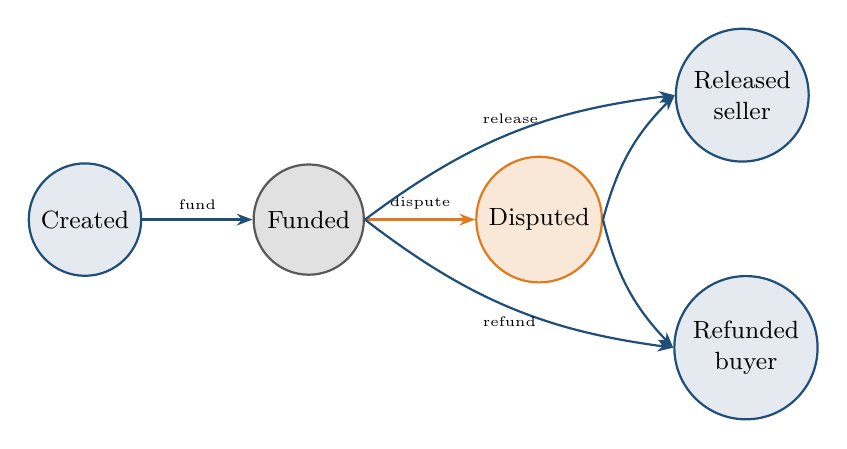
\begin{tikzpicture}[node distance=8mm and 14mm,font=\scriptsize]
  \node[node-state,node-state-normal] (c) {Created};
  \node[node-state,node-state-transition,right=of c] (f) {Funded};
  \node[node-state,node-state-alert,right=of f] (d) {Disputed};
  \node[node-state,node-state-normal,above right=4mm and 14mm of d] (rl) {Released\\seller};
  \node[node-state,node-state-normal,below right=4mm and 14mm of d] (rf) {Refunded\\buyer};
  \draw[arrow]       (c)  -- node[above,font=\tiny]{fund} (f);
  \draw[arrow-alert] (f)  -- node[above,font=\tiny]{dispute} (d);
  \draw[arrow]       (f.east) to[bend left=15]  node[above,font=\tiny]{release} (rl.west);
  \draw[arrow]       (f.east) to[bend right=15] node[below,font=\tiny]{refund}  (rf.west);
  \draw[arrow]       (d.east) to[bend left=15]  (rl.west);
  \draw[arrow]       (d.east) to[bend right=15] (rf.west);
\end{tikzpicture}
\vspace{1mm}
\small \textbf{Created $\to$ Funded} 只能一次；\textbf{Funded / Disputed $\to$ Released | Refunded} 是终态不可逆。
\srcnote{contracts/Escrow.sol:13--19 enum；:67--82 fund；:85--107 release/refund/dispute}
\end{frame}

\begin{frame}{业务流程映射：合约状态 vs 订单生命周期}
\begin{tabular}{@{}lll@{}}
\toprule
合约状态     & 订单状态        & 触发动作 \\
\midrule
Created      & 已下单未支付    & 合约部署完成 \\
Funded       & 已支付待发货    & 买家 fundWithOrderID \\
（链下）     & 商家发货 / 物流  & 链下流程，不影响合约 \\
Released     & 已完成          & 买家 / 仲裁人 release \\
Refunded     & 已退款          & 卖家 / 仲裁人 refund \\
Disputed     & 售后争议         & 买家或卖家 dispute \\
\bottomrule
\end{tabular}
\vspace{2mm}
\small 链上只记"钱在谁那里"，订单详情、物流、对账都在链下完成。\\
合约的不变式 = 业务的最低承诺。
\srcnote{contracts/README.md:31--36 合约不变式}
\end{frame}

% ============================================================
\section{链上对账与最终一致性}
% ============================================================

\begin{frame}{链是异步的：四个时间锚点}
\begin{tikzpicture}[font=\scriptsize]
  \draw[arrow,thick] (0,0) -- (11,0);
  \foreach \x/\name in {0.5/调用,3/打包,6/上链,9/N 确认} {
    \draw[cMain] (\x,-0.1) -- (\x,0.15);
    \node[font=\tiny,above,cMain] at (\x,0.15) {\name};
  }
  \node[font=\tiny,below,cGray] at (0.5,-0.1) {0s};
  \node[font=\tiny,below,cGray] at (3,-0.1)   {12--15s};
  \node[font=\tiny,below,cGray] at (6,-0.1)   {30--60s};
  \node[font=\tiny,below,cGray] at (9,-0.1)   {6 块 $\approx$ 90s};
\end{tikzpicture}
\vspace{4mm}
\begin{itemize}
  \item \textbf{0s 调用}：用户钱包广播 tx 到内存池。
  \item \textbf{12--15s 打包}：矿工 / validator 把 tx 装进区块。
  \item \textbf{30--60s 上链}：1 个确认完成。
  \item \textbf{90s N 确认}：6 个确认抗 reorg，金额越大 N 越大。
\end{itemize}
\small 业务侧客服话术："等待区块确认（通常 30--60s）"。
\srcnote{service/web3/listener.go:177--230 connectAndServe head 推进}
\end{frame}

\begin{frame}{listener 的三项基本功：重连 / catch-up / 幂等}
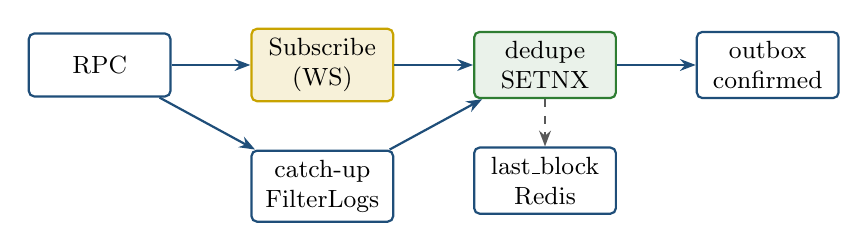
\begin{tikzpicture}[node distance=6mm and 10mm,font=\scriptsize]
  \node[node-box] (rpc) {RPC};
  \node[node-box,right=of rpc,node-warn] (sub) {Subscribe\\(WS)};
  \node[node-box,below=of sub] (cu)  {catch-up\\FilterLogs};
  \node[node-box,right=of sub,node-ok] (dd) {dedupe\\SETNX};
  \node[node-box,right=of dd]  (ob) {outbox\\confirmed};
  \node[node-box,below=of dd]  (lb) {last\_block\\Redis};
  \draw[arrow] (rpc) -- (sub);
  \draw[arrow] (rpc) -- (cu);
  \draw[arrow] (sub) -- (dd);
  \draw[arrow] (cu)  -- (dd);
  \draw[arrow] (dd)  -- (ob);
  \draw[arrow-async] (dd.south) -- (lb.north);
\end{tikzpicture}
\vspace{2mm}
\begin{itemize}
  \item 启动 / 重连后先 \texttt{catchUp(last+1, head)} 把停机漏掉的事件补齐。
  \item 每条 log 落 outbox 之前过 \texttt{web3:event:\{txhash\}:\{logindex\}} SETNX 去重。
  \item 处理完一条就 \texttt{saveLastBlock}，重启不会重做已成功的事件。
\end{itemize}
\srcnote{service/web3/listener.go:232--248 catchUp}
\srcnote{service/web3/listener.go:296--301 dedupeKey 设计；:316--326 tryClaim SETNX}
\end{frame}

\begin{frame}{容错边界 + outbox 接入最终一致体系}
\begin{tabular}{@{}lll@{}}
\toprule
异常       & 行为                              & 业务影响 \\
\midrule
RPC 断连     & 指数退避 1s $\to$ 60s 重连         & 短暂延迟，不掉单 \\
进程重启     & catchUp 从 last\_block+1 回放      & 不掉单 \\
log.Removed  & reorg log 跳过                    & 依赖 SETNX 兜底 \\
重复事件     & SETNX 72h，已处理 return          & 不重复推进订单 \\
\bottomrule
\end{tabular}
\vspace{1mm}
\small 复用 deck 04 outbox 总线，新增 \texttt{web3.payment.pending} / \texttt{web3.payment.confirmed} 两类事件，下游按 routing\_key 订阅；和传统支付\textbf{走同一条总线}，对账可复用。
\srcnote{service/web3/listener.go:155--175 重试；:218--221 reorg 跳过；:25--31 dedupe TTL}
\srcnote{service/payment\_crypto.go:129--148 事务内写 outbox web3.payment.pending}
\end{frame}

% ============================================================
\section{钱包签名验签：EIP-191 personal\_sign}
% ============================================================

\begin{frame}{为什么不能把私钥交给后端}
\begin{itemize}
  \item 私钥 = 钱包的全部，给了后端就不再是"用户的钱包"。
  \item 业界标准：让钱包对一段后端给定的消息签名，后端 \texttt{ecrecover} 反推地址。
  \item 业务收益：
  \begin{itemize}
    \item 不可否认：地址匹配 = 用户授权过；
    \item 零私钥泄漏面：签名过程发生在钱包客户端内部；
    \item 钓鱼防护：消息明文人类可读，用户在弹窗里能看到自己在签什么。
  \end{itemize}
\end{itemize}
\srcnote{pkg/web3/signature/verify.go:1--14 包注释设计意图}
\end{frame}

\begin{frame}{签名消息模板：把 chainID / orderID / nonce 都钉进去}
\begin{tikzpicture}[node distance=3mm,font=\scriptsize]
  \node[node-box,minimum width=75mm] (m) {\texttt{gomall:paydown:order=\{id\}:nonce=\{n\}:chain=\{cid\}}};
  \node[node-box,below=of m,minimum width=75mm,node-warn] (h) {EIP-191: keccak256("\textbackslash x19Ethereum Signed Message:\textbackslash n<len>" + msg)};
  \node[node-box,below=of h,minimum width=75mm,node-ok] (s) {ecrecover(hash, sig) $\to$ address vs 钱包地址};
  \draw[arrow] (m) -- (h);
  \draw[arrow] (h) -- (s);
\end{tikzpicture}
\vspace{1mm}
\small \textbf{chainID} 入消息防跨链重放；\textbf{orderID + nonce} 绑定订单 + 防重放；前缀 "gomall:paydown:" 让用户在钱包弹窗能识别；\textbf{v 值} 0/1 或 27/28 需归一化，地址比较 EIP-55 大小写无关。
\srcnote{service/payment\_crypto.go:39--46 signMessageTemplate}
\srcnote{pkg/web3/signature/verify.go:31--67 VerifyPersonalSign（含 v 规整）}
\end{frame}


% ============================================================
\section{业务边界、风险与角色关心}
% ============================================================

\begin{frame}{Web3 业务码与客服话术}
\begin{tabular}{@{}lll@{}}
\toprule
业务码              & 含义                  & 客服话术 \\
\midrule
W3-NONCE-EXPIRED    & nonce 5min 过期或被消费 & "请重新发起支付" \\
W3-SIG-INVALID      & 签名地址与提交不匹配   & "请用绑定钱包重试" \\
W3-PENDING          & 链上未确认             & "等待区块确认（约 30--60s）" \\
W3-AMOUNT-MISMATCH  & 链上金额 $\ne$ 订单金额 & "金额异常，已挂起人工" \\
W3-REORG            & 链上 reorg 撤销         & "网络回滚，已退款" \\
\bottomrule
\end{tabular}
\vspace{2mm}
\small 业务码不暴露技术细节，但要给客服\textbf{足够区分}的话术。\\
W3-PENDING vs W3-NONCE-EXPIRED 看起来都是"再试一次"，应对策略完全不同。
\srcnote{repository/cache/web3.go:29--33 ErrWeb3NonceMissing / ErrWeb3NonceMismatch}
\end{frame}

\begin{frame}{各角色关心}
\begin{tabular}{@{}lll@{}}
\toprule
角色   & 关心               & 看哪里 \\
\midrule
用户   & 钱安全吗            & 合约审计报告 + 多签 + 退款流程 \\
商家   & 何时到账            & 链上确认数 + release 时机 \\
客服   & 链上失败咋办        & W3-* 业务码对应处理 SOP \\
SRE    & 节点稳定否          & RPC 多源切换 + listener 健康 \\
法务   & 合规边界            & KYC + 多签 + 司法管辖 \\
财务   & 链上链下并存对账     & outbox + 链上事件 + 法币入账 \\
\bottomrule
\end{tabular}
\vspace{2mm}
\srcnote{contracts/README.md:88--103 安全注意 + 部署参数（多签建议）}
\end{frame}

\begin{frame}{业务边界：接哪条链、接哪些币、谁出 gas}
\begin{tabular}{@{}lll@{}}
\toprule
维度    & 选项                  & 对业务的影响 \\
\midrule
链       & 以太坊主网            & gas 贵、确认慢、用户基数大 \\
         & Polygon / Optimism / Arbitrum (L2) & gas 便宜，确认快，跨链桥风险 \\
币       & ETH / MATIC 原生币    & 价格波动直接传导到订单金额 \\
         & USDC / USDT 稳定币    & 电商更适合，需要 ERC-20 路径 \\
gas      & 用户自付              & gomall 当前路线，门槛偏高 \\
         & 商家补贴 / 平台垫付   & 体验好，需要 gas 钱包管理 \\
\bottomrule
\end{tabular}
\vspace{2mm}
\small 链 / 币 / gas 三选一组合，业务侧通常先选 L2 + 稳定币 + 用户自付出 gas 做 MVP。
\srcnote{service/payment\_crypto.go:41 signMessageTemplate 已为多 chainID 留接口}
\end{frame}

\begin{frame}{风险与合规}
\small
\begin{itemize}
  \item \textbf{合约不可改}：bug 只能换合约 + 链下迁移；缓解：第三方审计 + 充分单测。
  \item \textbf{私钥丢失}：链上无"重置密码"；缓解：仲裁人确凿身份核实后 refund 到新地址。
  \item \textbf{gas 飙升}：mainnet 拥堵 tx 失败；缓解：默认 L2，fallback mainnet 明确提示。
  \item \textbf{Reorg}：浅确认下 release 可能撤销；缓解：大额提高 N 确认 + outbox 兜底。
  \item \textbf{AML / OFAC}：制裁名单地址必须拒绝；缓解：验签阶段加地址过滤。
  \item \textbf{现状}：合约源 + Go binding 已在 feat/web3-escrow PR，\textbf{未上链}。
\end{itemize}
\srcnote{service/web3/listener.go:218--221 reorg log 跳过；contracts/README.md:88--103}
\end{frame}

% ============================================================
\section{运营连续性：和传统支付并存}
% ============================================================

\begin{frame}{和传统第三方支付的对账如何并存}
\begin{tikzpicture}[node distance=4mm and 8mm,font=\scriptsize]
  \node[node-box] (ord)  {订单服务};
  \node[node-box,above right=2mm and 14mm of ord,node-ok]  (fiat) {fiat\\paydown};
  \node[node-box,below right=2mm and 14mm of ord,node-warn] (w3) {web3\\paydown};
  \node[node-box,right=20mm of ord,node-state-transition] (ob)  {outbox\\总线};
  \node[node-box,right=of ob]  (rec) {对账\\任务};
  \draw[arrow] (ord) -- (fiat);
  \draw[arrow] (ord) -- (w3);
  \draw[arrow] (fiat) -- (ob);
  \draw[arrow] (w3)   -- (ob);
  \draw[arrow] (ob) -- (rec);
\end{tikzpicture}
\vspace{3mm}
\begin{itemize}
  \item 两条支付通道\textbf{共用同一条 outbox 总线}，事件统一格式。
  \item 对账任务按 \texttt{order\_id} 维度做 join：链上 confirmed event + 传统支付回调。
  \item 财务报表里区分 channel 字段：\texttt{fiat / web3-eth / web3-usdc}。
\end{itemize}
\srcnote{service/payment\_crypto.go:129--148 事务内写 outbox 保证最终一致}
\end{frame}

\begin{frame}{大额订单的多签托管路线图}
\begin{itemize}
  \item \textbf{阶段 1（MVP）}：平台单签 arbiter，适合小额 + 内测。
  \item \textbf{阶段 2}：Gnosis Safe 2-of-3，平台 + 商户联盟 + 第三方仲裁机构。
  \item \textbf{阶段 3}：链下结合 DAO 投票，大额争议走治理代币投票决定。
\end{itemize}
\vspace{2mm}
\begin{tabular}{@{}lll@{}}
\toprule
阶段 & arbiter 形态        & 适用金额上限 \\
\midrule
1    & 平台 EOA           & 等值 \$100 以内 \\
2    & 2-of-3 多签        & 等值 \$10{,}000 以内 \\
3    & DAO 治理           & 超大额 / 跨组织 \\
\bottomrule
\end{tabular}
\srcnote{contracts/README.md:96--103 arbiter 推荐用 Gnosis Safe / DAO}
\end{frame}

\begin{frame}{从技术决策回看业务依据}
\begin{tabular}{@{}ll@{}}
\toprule
技术选择                        & 业务依据 \\
\midrule
EIP-191 personal\_sign          & 钱包弹窗能让用户看到明文，钓鱼可识别 \\
nonce 走 Redis + Lua            & 防重放门槛要原子，单实例语义不够 \\
合约 emit PaymentConfirmed       & 链下 listener 只需订阅一个 event，对账简单 \\
listener 写 outbox 而非直推订单 & 复用 deck 04 的最终一致体系 \\
SETNX 事件级幂等                & reorg / 重连 / 重启都不会重复推进订单 \\
arbiter 走多签路线              & 单签平台跑路风险无法对外解释 \\
\bottomrule
\end{tabular}
\srcnote{routes/router.go:111--114 三选一接入位}
\end{frame}

\begin{frame}{业务侧的最终目标}
\begin{itemize}
  \item 用户：钱进托管前订单一定 pending；钱进合约后订单一定推进，不会"先付款后失踪"。
  \item 商家：链上 release 后 30s 内系统通知到账，物流可发。
  \item 客服：拿到 W3-* 业务码就能定位问题，不需要懂链。
  \item SRE：listener / RPC / Redis / outbox 各自有健康指标，能独立排障。
\end{itemize}
\keypoint{Web3 支付的业务价值不在"潮"，在于\textbf{把"第三方"从"中介机构"换成"可审计的代码"}。}
\end{frame}

% ============================================================
\appendix
% ============================================================

\begin{frame}{面试 Q\&A（上）}
\textbf{Q1}：链 reorg 导致已 release 的资金被撤销怎么办？\\
\hspace{4mm}\small A：金额越大 N 确认越多（大额至少 12--20 块）；listener 监听 \texttt{lg.Removed} 跳过 reorg log，订单状态不会被错误推进；若已发货，走对账兜底 + 仲裁人介入。

\vspace{2mm}
\textbf{Q2}：用户钱包私钥丢了订单怎么处理？\\
\hspace{4mm}\small A：链上没有"重置密码"。若资金还在 Funded 态，可通过仲裁人确凿身份核实后走 refund 到用户提交的新地址；若已 Released 给商家，则只能走链下补偿。

\vspace{2mm}
\textbf{Q3}：gas 飙升导致用户支付 tx 失败怎么补救？\\
\hspace{4mm}\small A：默认路由到 L2；nonce 5min 内允许用户重新提交带更高 gas 的 tx；超时则重新颁发 nonce + 签名。
\end{frame}

\begin{frame}{面试 Q\&A（下）}
\textbf{Q4}：和传统第三方支付的对账如何并存？\\
\hspace{4mm}\small A：两条通道都把支付事件落到同一条 outbox 总线，事件加 channel 字段（fiat / web3-eth / web3-usdc）。对账任务按 \texttt{order\_id} join 法币入账记录 + 链上 confirmed event。

\vspace{2mm}
\textbf{Q5}：Layer 2 vs 主网怎么选？\\
\hspace{4mm}\small A：L2 适合高频小额、对延迟敏感；主网适合大额、对最终性敏感。MVP 用 L2 + 稳定币 + 用户自付 gas，长期支持双链并行，由订单金额自动路由。

\vspace{2mm}
\textbf{Q6}：多签 arbiter 该谁来当？\\
\hspace{4mm}\small A：MVP 用平台单签便于上线；进入正式运营后必须升级 2-of-3 多签（平台 + 商户联盟 + 第三方仲裁），大额订单进一步走 DAO 投票。单签平台跑路风险无法对外解释。
\end{frame}

\begin{frame}{代码位置一览（feat/web3-* 三件套）}
\small
\begin{description}
  \item[Escrow 合约]\srcnote{contracts/Escrow.sol:7--113}
  \item[部署文档]\srcnote{contracts/README.md:1--104}
  \item[Go binding 占位]\srcnote{pkg/web3/escrow/escrow.go:14--80}
  \item[钱包验签]\srcnote{pkg/web3/signature/verify.go:31--82}
  \item[Nonce / 验签业务]\srcnote{service/payment\_crypto.go:49--160}
  \item[Web3 Redis 协议]\srcnote{repository/cache/web3.go:21--101}
  \item[链上事件 listener]\srcnote{service/web3/listener.go:108--326}
  \item[API handler + router]\srcnote{api/v1/paydown\_crypto.go:16--52；routes/router.go:111--114}
\end{description}
\keypoint{现状：合约 + binding 已在 feat/web3-escrow PR，\textbf{未上链}；上线前需第三方审计。}
\end{frame}

\end{document}
